% Options for packages loaded elsewhere
% Options for packages loaded elsewhere
\PassOptionsToPackage{unicode}{hyperref}
\PassOptionsToPackage{hyphens}{url}
%
\documentclass[
  ignorenonframetext,
]{beamer}
\newif\ifbibliography
\usepackage{pgfpages}
\setbeamertemplate{caption}[numbered]
\setbeamertemplate{caption label separator}{: }
\setbeamercolor{caption name}{fg=normal text.fg}
\beamertemplatenavigationsymbolsempty
% remove section numbering
\setbeamertemplate{part page}{
  \centering
  \begin{beamercolorbox}[sep=16pt,center]{part title}
    \usebeamerfont{part title}\insertpart\par
  \end{beamercolorbox}
}
\setbeamertemplate{section page}{
  \centering
  \begin{beamercolorbox}[sep=12pt,center]{section title}
    \usebeamerfont{section title}\insertsection\par
  \end{beamercolorbox}
}
\setbeamertemplate{subsection page}{
  \centering
  \begin{beamercolorbox}[sep=8pt,center]{subsection title}
    \usebeamerfont{subsection title}\insertsubsection\par
  \end{beamercolorbox}
}
% Prevent slide breaks in the middle of a paragraph
\widowpenalties 1 10000
\raggedbottom
\AtBeginPart{
  \frame{\partpage}
}
\AtBeginSection{
  \ifbibliography
  \else
    \frame{\sectionpage}
  \fi
}
\AtBeginSubsection{
  \frame{\subsectionpage}
}
\usepackage{iftex}
\ifPDFTeX
  \usepackage[T1]{fontenc}
  \usepackage[utf8]{inputenc}
  \usepackage{textcomp} % provide euro and other symbols
\else % if luatex or xetex
  \usepackage{unicode-math} % this also loads fontspec
  \defaultfontfeatures{Scale=MatchLowercase}
  \defaultfontfeatures[\rmfamily]{Ligatures=TeX,Scale=1}
\fi
\usepackage{lmodern}

\usetheme[]{metropolis}
\ifPDFTeX\else
  % xetex/luatex font selection
\fi
% Use upquote if available, for straight quotes in verbatim environments
\IfFileExists{upquote.sty}{\usepackage{upquote}}{}
\IfFileExists{microtype.sty}{% use microtype if available
  \usepackage[]{microtype}
  \UseMicrotypeSet[protrusion]{basicmath} % disable protrusion for tt fonts
}{}
\makeatletter
\@ifundefined{KOMAClassName}{% if non-KOMA class
  \IfFileExists{parskip.sty}{%
    \usepackage{parskip}
  }{% else
    \setlength{\parindent}{0pt}
    \setlength{\parskip}{6pt plus 2pt minus 1pt}}
}{% if KOMA class
  \KOMAoptions{parskip=half}}
\makeatother


\usepackage{longtable,booktabs,array}
\usepackage{calc} % for calculating minipage widths
\usepackage{caption}
% Make caption package work with longtable
\makeatletter
\def\fnum@table{\tablename~\thetable}
\makeatother
\usepackage{graphicx}
\makeatletter
\newsavebox\pandoc@box
\newcommand*\pandocbounded[1]{% scales image to fit in text height/width
  \sbox\pandoc@box{#1}%
  \Gscale@div\@tempa{\textheight}{\dimexpr\ht\pandoc@box+\dp\pandoc@box\relax}%
  \Gscale@div\@tempb{\linewidth}{\wd\pandoc@box}%
  \ifdim\@tempb\p@<\@tempa\p@\let\@tempa\@tempb\fi% select the smaller of both
  \ifdim\@tempa\p@<\p@\scalebox{\@tempa}{\usebox\pandoc@box}%
  \else\usebox{\pandoc@box}%
  \fi%
}
% Set default figure placement to htbp
\def\fps@figure{htbp}
\makeatother





\setlength{\emergencystretch}{3em} % prevent overfull lines

\providecommand{\tightlist}{%
  \setlength{\itemsep}{0pt}\setlength{\parskip}{0pt}}



 


\setbeamerfont{title}{size=\large}
\usepackage{hyperref}
\setbeamertemplate{footline}[frame number]
\usepackage{tikz}
\usetikzlibrary{arrows.meta, positioning, shapes.geometric, fit, backgrounds, calc}
\usepackage{booktabs}
\usepackage{xcolor}
\definecolor{mblue}{RGB}{35,55,100}
\makeatletter
\@ifpackageloaded{caption}{}{\usepackage{caption}}
\AtBeginDocument{%
\ifdefined\contentsname
  \renewcommand*\contentsname{Table of contents}
\else
  \newcommand\contentsname{Table of contents}
\fi
\ifdefined\listfigurename
  \renewcommand*\listfigurename{List of Figures}
\else
  \newcommand\listfigurename{List of Figures}
\fi
\ifdefined\listtablename
  \renewcommand*\listtablename{List of Tables}
\else
  \newcommand\listtablename{List of Tables}
\fi
\ifdefined\figurename
  \renewcommand*\figurename{Figure}
\else
  \newcommand\figurename{Figure}
\fi
\ifdefined\tablename
  \renewcommand*\tablename{Table}
\else
  \newcommand\tablename{Table}
\fi
}
\@ifpackageloaded{float}{}{\usepackage{float}}
\floatstyle{ruled}
\@ifundefined{c@chapter}{\newfloat{codelisting}{h}{lop}}{\newfloat{codelisting}{h}{lop}[chapter]}
\floatname{codelisting}{Listing}
\newcommand*\listoflistings{\listof{codelisting}{List of Listings}}
\makeatother
\makeatletter
\makeatother
\makeatletter
\@ifpackageloaded{caption}{}{\usepackage{caption}}
\@ifpackageloaded{subcaption}{}{\usepackage{subcaption}}
\makeatother

\usepackage{bookmark}
\IfFileExists{xurl.sty}{\usepackage{xurl}}{} % add URL line breaks if available
\urlstyle{same}
\hypersetup{
  pdfauthor={Giorgio Arcara},
  hidelinks,
  pdfcreator={LaTeX via pandoc}}


\author{Giorgio Arcara}
\date{}

\begin{document}


\begin{frame}
\title{Metodologia della Ricerca Clinica\\
\vspace{0.5em}
{\normalsize \textbf{11. Disegni di Ricerca Clinica}}}
\author{Giorgio Arcara,\\ Università di Padova \\ IRCCS San Camillo, Venezia}
\titlegraphic{
\vspace*{7cm}
\includegraphics[scale=0.15]{Figures/LogoSanCamilloIRCCS_Unipd_alpha.png}
\hfill \includegraphics[scale=0.15]{Figures/CC_license_3_0.png}
}
\maketitle
\end{frame}

\section{La Gerarchia delle Evidenze}\label{la-gerarchia-delle-evidenze}

\begin{frame}{EBM Pyramid: il filo conduttore del corso}
\phantomsection\label{ebm-pyramid-il-filo-conduttore-del-corso}
% [IMMAGINE SUGGERITA: classica piramide EBM a 6 livelli con colori graduali]
\begin{center}
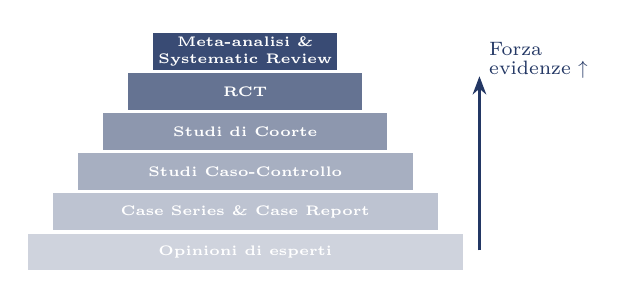
\begin{tikzpicture}[scale=0.85, font=\tiny]
  \foreach \i/\lbl/\shade in {
    0/{Opinioni di esperti}/22,
    1/{Case Series \& Case Report}/30,
    2/{Studi Caso-Controllo}/40,
    3/{Studi di Coorte}/52,
    4/{RCT}/70,
    5/{Meta-analisi \& \\ Systematic Review}/90
  }{
    \pgfmathsetmacro{\w}{6.5 - \i*0.75}
    \pgfmathsetmacro{\y}{\i*0.6}
    \fill[mblue!\shade] (-\w/2, \y) rectangle (\w/2, \y+0.55);
    \node[white, font=\tiny\bfseries, align=center] at (0, \y+0.27) {\lbl};
  }
  \node[right, font=\scriptsize, mblue] at (3.5, 3.3) {Forza};
  \node[right, font=\scriptsize, mblue] at (3.5, 3.0) {evidenze $\uparrow$};
  \draw[-{Stealth}, mblue, thick] (3.5, 0.3) -- (3.5, 2.9);
\end{tikzpicture}
\end{center}
\vspace{-0.3em}
\small La piramide \textbf{Evidence Based Medicine} (EBM) pyramid organizza i disegni per \textbf{forza delle evidenze prodotte}.
\end{frame}

\section{1.1 Tassonomia Generale}\label{tassonomia-generale}

\begin{frame}{Osservazionale vs Interventistico}
\phantomsection\label{osservazionale-vs-interventistico}
\begin{center}
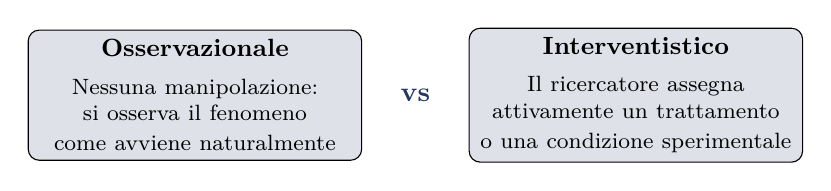
\begin{tikzpicture}[
  box/.style={draw, rounded corners=4pt, fill=mblue!15, text width=4cm,
              align=center, minimum height=1.4cm, font=\small},
]
\node[box] (obs) at (-2.8,0) {
  \textbf{Osservazionale}\\[4pt]
  \footnotesize Nessuna manipolazione:\\
  si osserva il fenomeno\\come avviene naturalmente
};
\node[box] (int) at (2.8,0) {
  \textbf{Interventistico}\\[4pt]
  \footnotesize Il ricercatore assegna\\
  attivamente un trattamento\\
  o una condizione sperimentale
};
\node[font=\normalsize\bfseries, mblue] at (0,0) {vs};
\end{tikzpicture}
\end{center}
\vspace{0.4em}
\begin{columns}
\column{0.5\textwidth}
\footnotesize \textbf{Esempio:} associazione tra punteggi ad un test di screening e probabilità sviluppo demenza.
\column{0.5\textwidth}
\footnotesize \textbf{Esempio:} training cognitivo computerizzato vs.\ lista d'attesa in pazienti con MCI.
\end{columns}
\end{frame}

\begin{frame}{Posso randomizzare?}
\phantomsection\label{posso-randomizzare}
\begin{center}
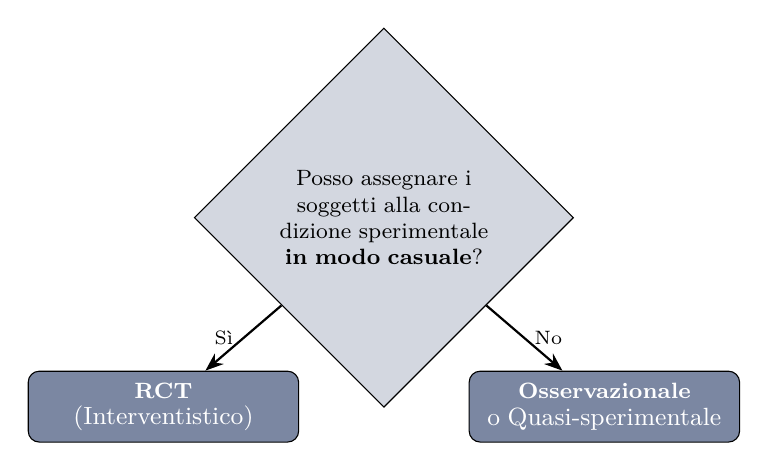
\begin{tikzpicture}[
  dec/.style={diamond, draw, fill=mblue!20, text width=3.2cm, align=center,
              font=\footnotesize, inner sep=3pt},
  term/.style={rectangle, rounded corners, draw, fill=mblue!60, text=white,
               text width=3.2cm, align=center, font=\footnotesize, minimum height=0.9cm},
  arr/.style={-{Stealth}, thick}
]
\node[dec] (q1) at (0,2.4) {Posso assegnare i soggetti alla condizione sperimentale \textbf{in modo casuale}?};
\node[term] (yes) at (-2.8,0) {\textbf{RCT}\\\small (Interventistico)};
\node[term] (no)  at ( 2.8,0) {\textbf{Osservazionale}\\\small o Quasi-sperimentale};
\draw[arr] (q1) -- node[left,  font=\scriptsize]{Sì} (yes);
\draw[arr] (q1) -- node[right, font=\scriptsize]{No} (no);
\end{tikzpicture}
\end{center}
\vspace{0.3em}
\small In neuropsicologia e psicologia clinica la randomizzazione spesso non è praticabile: \textbf{la patologia è già presente}, i vincoli etici lo impediscono, o le risorse sono insufficienti.
\end{frame}

\begin{frame}{Spiegazioni alternative}
\phantomsection\label{spiegazioni-alternative}
Un modo per pensare la diversa forza di evidenze disponibili è relativa
all'interpretazione dei risultati.

Negli studi osservazionali esiste una più grande possibilità di
\textbf{spiegazioni alternative} dei risultati osservati. Questo perché
\textbf{confounders} noti oppure no, potrebbero avere influenzato i
risulatti. \vfill \small \emph{confounder}: variabile associata alla
variabile di interesse che può avere influenzato i risultati
\end{frame}

\section{1.2 Dimensione Temporale negli studi
osservazionali}\label{dimensione-temporale-negli-studi-osservazionali}

\begin{frame}{Retrospettivo vs Prospettico (osservazionali)}
\phantomsection\label{retrospettivo-vs-prospettico-osservazionali}
\begin{center}
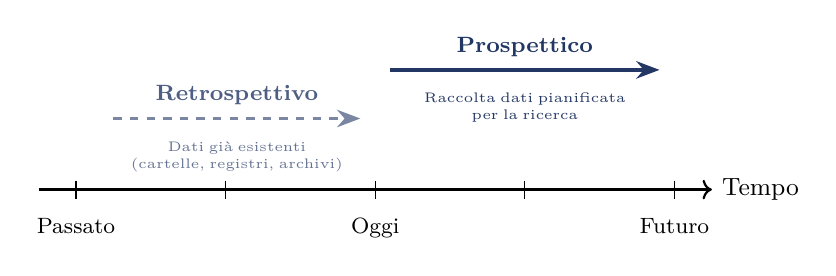
\begin{tikzpicture}[scale=0.95]
  \draw[thick, ->] (-4.5,0) -- (4.5,0) node[right,font=\small]{Tempo};
  \foreach \x in {-4,-2,0,2,4}
    \draw (\x,0.12)--(\x,-0.12);
  \node[below,font=\footnotesize] at (-4,-0.25) {Passato};
  \node[below,font=\footnotesize] at ( 0,-0.25) {Oggi};
  \node[below,font=\footnotesize] at ( 4,-0.25) {Futuro};

  \draw[-{Stealth}, dashed, mblue!60, very thick] (-3.5,0.95) -- (-0.2,0.95);
  \node[above,font=\footnotesize,mblue!80] at (-1.85, 1.00) {\textbf{Retrospettivo}};
  \node[below,font=\tiny,mblue!70,text width=3.5cm,align=center] at (-1.85,0.77)
    {Dati già esistenti\\(cartelle, registri, archivi)};

  \draw[-{Stealth}, mblue, very thick] (0.2,1.6) -- (3.8,1.6);
  \node[above,font=\footnotesize,mblue] at (2.0,1.65) {\textbf{Prospettico}};
  \node[below,font=\tiny,mblue,text width=3.5cm,align=center] at (2.0,1.42)
    {Raccolta dati pianificata\\per la ricerca};
\end{tikzpicture}
\end{center}
\vspace{0.4em}
\begin{columns}
\column{0.5\textwidth}
\small \textbf{Retrospettivo}: rapido ed economico; rischio di \emph{bias di selezione} e di misura (dati non raccolti per la ricerca).
\column{0.5\textwidth}
\small \textbf{Prospettico}: costoso e lento; maggiore controllo su qualità e completezza dei dati.
\end{columns}
\end{frame}

\begin{frame}{Studio Cross-Sectional (osservazionali)}
\phantomsection\label{studio-cross-sectional-osservazionali}
\begin{center}
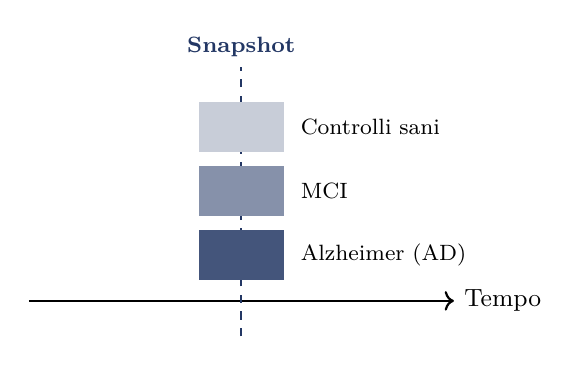
\begin{tikzpicture}[scale=0.9]
  \draw[thick,->] (-1,0) -- (5,0) node[right,font=\small]{Tempo};
  \draw[thick,mblue,dashed] (2,-0.5) -- (2,3.3)
    node[above,font=\footnotesize,mblue]{\textbf{Snapshot}};
  \foreach \y/\lbl/\shade in {
    0.3/{Alzheimer (AD)}/85,
    1.2/MCI/55,
    2.1/{Controlli sani}/25
  }{
    \fill[mblue!\shade] (1.4,\y) rectangle (2.6,\y+0.7);
    \node[right,font=\footnotesize] at (2.7,\y+0.35) {\lbl};
  }
\end{tikzpicture}
\end{center}
\vspace{-0.3em}

\small

\begin{itemize}
\tightlist
\item
  Tutti i gruppi misurati in un \textbf{unico momento temporale}
\item
  Economico, rapido
\item
  Utile per stime di \textbf{prevalenza} e per \textbf{generare ipotesi}
\item
  \textbf{Limite principale}: non permette di tracciare traiettorie
  individuali né inferenze causali solide
\end{itemize}

\emph{Esempio: confronto prestazioni mnestiche tra Controlli, MCI e AD
su un singolo time point}
\end{frame}

\begin{frame}{Studio Longitudinale (osservazionali)}
\phantomsection\label{studio-longitudinale-osservazionali}
\begin{center}
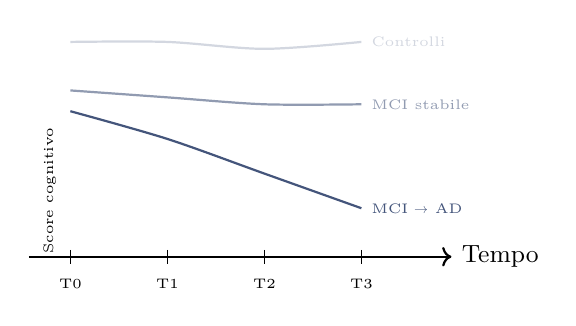
\begin{tikzpicture}[scale=0.88]
  \draw[thick,->] (-0.3,0) -- (5.8,0) node[right,font=\small]{Tempo};
  \foreach \x/\lbl in {0.3/T0, 1.7/T1, 3.1/T2, 4.5/T3}{
    \draw (\x,0.1)--(\x,-0.1);
    \node[below,font=\tiny] at (\x,-0.18) {\lbl};
  }
  \draw[thick, mblue!85] plot[smooth]
    coordinates {(0.3,2.1)(1.7,1.7)(3.1,1.2)(4.5,0.7)}
    node[right,font=\tiny]{MCI $\to$ AD};
  \draw[thick, mblue!50] plot[smooth]
    coordinates {(0.3,2.4)(1.7,2.3)(3.1,2.2)(4.5,2.2)}
    node[right,font=\tiny]{MCI stabile};
  \draw[thick, mblue!20] plot[smooth]
    coordinates {(0.3,3.1)(1.7,3.1)(3.1,3.0)(4.5,3.1)}
    node[right,font=\tiny]{Controlli};
  \node[left,font=\tiny,rotate=90] at (0.0,2.0) {Score cognitivo};
\end{tikzpicture}
\end{center}
\vspace{-0.4em}

\small

\begin{itemize}
\tightlist
\item
  Gli stessi soggetti vengono seguiti nel tempo (\textbf{follow-up}
  ripetuto)
\item
  Permette di studiare \textbf{traiettorie individuali} e cambiamento
  intra-individuale
\item
  Costoso e lento; soggetto ad \textbf{attrition} (abbandono) che può
  non essere casuale
\end{itemize}

\emph{Esempio: studio
\href{https://adni.loni.usc.edu/}{\underline{\textbf{ADNI}}} ---
monitoraggio annuale per predire conversione MCI \(\to\) AD}
\end{frame}

\begin{frame}{Cross-Sectional come primo passo}
\phantomsection\label{cross-sectional-come-primo-passo}
\begin{center}
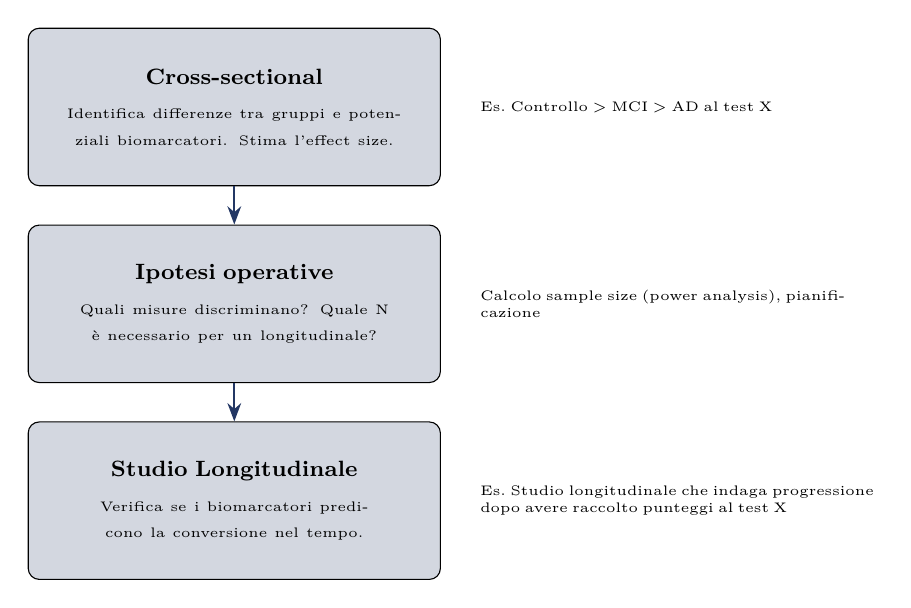
\begin{tikzpicture}[
  box/.style={draw, rounded corners, fill=mblue!20, text width=5cm,
              align=center, font=\footnotesize, minimum height=2cm},
  arr/.style={-{Stealth}, thick, mblue}
]
\node[box] (cs)   at (0, 5.0) {\textbf{Cross-sectional}\\[3pt]\tiny Identifica differenze tra gruppi e potenziali biomarcatori. Stima l'effect size.};
\node[box] (hyp)  at (0, 2.5) {\textbf{Ipotesi operative}\\[3pt]\tiny Quali misure discriminano? Quale N è necessario per un longitudinale?};
\node[box] (long) at (0, 0.0) {\textbf{Studio Longitudinale}\\[3pt]\tiny Verifica se i biomarcatori predicono la conversione nel tempo.};
\draw[arr] (cs)  -- (hyp);
\draw[arr] (hyp) -- (long);
\node[right,font=\tiny,text width=5cm] at (3,5) {Es.\ Controllo > MCI > AD al test X};
\node[right,font=\tiny,text width=5cm] at (3,2.5) {Calcolo sample size (power analysis), pianificazione};
\node[right,font=\tiny,text width=5cm] at (3,0.0) {Es.\ Studio longitudinale che indaga progressione dopo avere raccolto punteggi al test X};
\end{tikzpicture}
\end{center}
\end{frame}

\begin{frame}{Studi di Coorte e Caso-Controllo}
\phantomsection\label{studi-di-coorte-e-caso-controllo}
\begin{columns}
\column{0.5\textwidth}
\textbf{Studio di Coorte}
\vspace{0.3em}

\footnotesize Si segue un gruppo (\emph{coorte}) nel tempo. Si confrontano esposti vs non esposti a un fattore.

\vspace{0.3em}
\emph{Es.} Pazienti con depressione vs controlli: chi sviluppa declino cognitivo entro 5 anni?

\vspace{0.3em}
\textbf{Pro}: ordine temporale chiaro\\
\textbf{Contro}: costoso, lungo, attrition

\column{0.5\textwidth}
\textbf{Studio Caso-Controllo}
\vspace{0.3em}

\footnotesize Si parte dall'\emph{outcome} (casi vs controlli senza la condizione) e si guarda retrospettivamente all'esposizione.

\vspace{0.3em}
\emph{Es.} Pazienti con ictus vs controlli: differenze nel profilo neuropsicologico pre-morboso (da cartelle)?

\vspace{0.3em}
\textbf{Pro}: efficiente per patologie rare\\
\textbf{Contro}: bias di selezione e recall
\end{columns}
\end{frame}

\section{1.3 RCT e Disegni
Sperimentali}\label{rct-e-disegni-sperimentali}

\begin{frame}{Il Randomized Controlled Trial (RCT)}
\phantomsection\label{il-randomized-controlled-trial-rct}
L'efficacia del trattamento è studiata tramite l'allocazione
\textbf{random} a due trattamenti: uno sperimentale e uno di controllo.
\end{frame}

\begin{frame}{Perché randomizzare?}
\phantomsection\label{perchuxe9-randomizzare}
\begin{itemize}
\tightlist
\item
  La randomizzazione \textbf{bilancia i confounders noti e ignoti} tra i
  gruppi, anche quelli che non abbiamo misurato
\item
  Senza randomizzazione, le differenze osservate potrebbero riflettere
  \textbf{differenze pre-esistenti} tra i gruppi (selection bias)
\end{itemize}

\vspace{0.5em}

\emph{Esempio: se i pazienti più motivati \emph{scelgono} il training
cognitivo, qualsiasi miglioramento osservato potrebbe essere dovuto alla
motivazione, non al training.}

\vspace{0.5em}
\end{frame}

\begin{frame}{Elementi fondamentali di un RCT di qualità}
\phantomsection\label{elementi-fondamentali-di-un-rct-di-qualituxe0}
\small

\begin{itemize}
\tightlist
\item
  Sequenza di randomizzazione con
  \href{https://pmc.ncbi.nlm.nih.gov/articles/PMC6022887/pdf/10.1177_0141076818776604.pdf}{\underline{\textbf{allocation concealment}}}
\item
  \textbf{Blinding}: singolo (paziente), doppio (+ valutatore), triplo
  (+ analista)
\item
  Analisi \textbf{intention-to-treat} (ITT) vs per-protocol
\item
  Controllo \textbf{adeguato}
\item
  Reporting secondo standard \textbf{CONSORT}
\end{itemize}

\vspace{0.2em}

\tiny Moher et al.~(2010). CONSORT 2010. \emph{BMJ} 340:c332.
\href{https://www.bmj.com/content/340/bmj.c332}{\underline{\textbf{Download Article}}}
\end{frame}

\begin{frame}{Tipi di Disegno RCT}
\phantomsection\label{tipi-di-disegno-rct}
\begin{center}
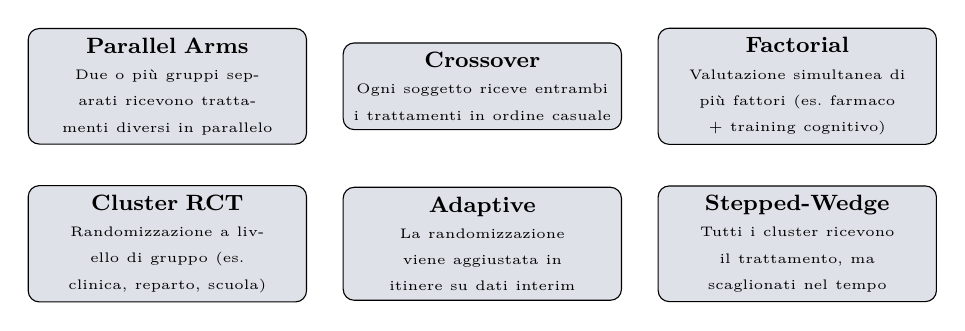
\begin{tikzpicture}[
  box/.style={draw, rounded corners, fill=mblue!15, text width=3.3cm,
              align=center, font=\footnotesize, minimum height=1.1cm},
]
\node[box] at (-6, 2) {\textbf{Parallel Arms}\\\tiny Due o più gruppi separati ricevono trattamenti diversi in parallelo};
\node[box] at ( -2,   2) {\textbf{Crossover}\\\tiny Ogni soggetto riceve entrambi i trattamenti in ordine casuale};
\node[box] at ( 2, 2) {\textbf{Factorial}\\\tiny Valutazione simultanea di più fattori (es.\ farmaco + training cognitivo)};
\node[box] at (-6, 0) {\textbf{Cluster RCT}\\\tiny Randomizzazione a livello di gruppo (es.\ clinica, reparto, scuola)};
\node[box] at ( -2, 0) {\textbf{Adaptive}\\\tiny La randomizzazione viene aggiustata in itinere su dati interim};
\node[box] at ( 2,0) {\textbf{Stepped-Wedge}\\\tiny Tutti i cluster ricevono il trattamento, ma scaglionati nel tempo};
\end{tikzpicture}
\end{center}
\end{frame}

\begin{frame}{Disegno RCT Parallel Arms}
\phantomsection\label{disegno-rct-parallel-arms}
% [IMMAGINE SUGGERITA: CONSORT flow diagram ufficiale]
\begin{center}
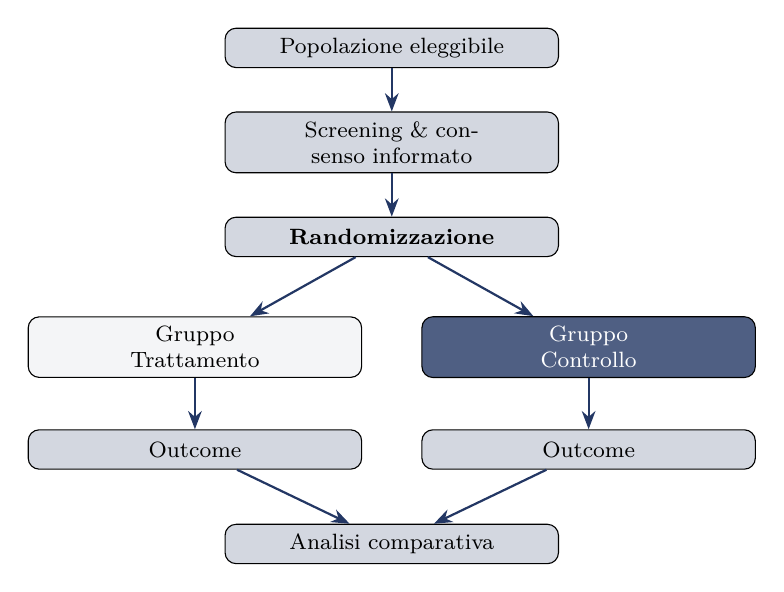
\begin{tikzpicture}[
  box/.style={draw, rounded corners, fill=mblue!20, text width=4cm,
              align=center, font=\footnotesize, minimum height=0.5cm},
  arr/.style={-{Stealth}, thick, mblue}
]
\node[box] (pop)  at (0, 4.2) {Popolazione eleggibile};
\node[box] (elig) at (0, 3.0) {Screening \& consenso informato};
\node[box] (rand) at (0, 1.8) {\textbf{Randomizzazione}};
\node[box, fill= mblue!05] (trt)  at (-2.5, 0.4) {Gruppo\\Trattamento};
\node[box, fill= mblue!80, text=white] (ctrl) at ( 2.5, 0.4) {Gruppo\\Controllo};
\node[box] (o1)   at (-2.5,-0.9) {Outcome};
\node[box] (o2)   at ( 2.5,-0.9) {Outcome};
\node[box] (anal) at (0,  -2.1) {Analisi comparativa};
\draw[arr] (pop)  -- (elig);
\draw[arr] (elig) -- (rand);
\draw[arr] (rand) -- (trt);
\draw[arr] (rand) -- (ctrl);
\draw[arr] (trt)  -- (o1);
\draw[arr] (ctrl) -- (o2);
\draw[arr] (o1)   -- (anal);
\draw[arr] (o2)   -- (anal);
\end{tikzpicture}
\end{center}
\end{frame}

\begin{frame}{RCT Parallel arms: note}
\phantomsection\label{rct-parallel-arms-note}
\begin{itemize}
\tightlist
\item
  Disegno più comune: due o più gruppi ricevono trattamenti diversi
  \textbf{in parallelo} per tutta la durata
\end{itemize}

\textbf{Vantaggi} - semplice da implementare, analizzare e interpretare

Importante tenere conto di:

\begin{itemize}
\tightlist
\item
  la variabilità inter-individuale richiede campioni ampi;
\item
  il \textbf{controllo attivo} (es.~attività motoria) è preferibile al
  no-treatment per controllare effetti aspecifici (es. aspettativa,
  coinvolgimento emotivo).
\end{itemize}
\end{frame}

\begin{frame}{Disegno RCT Crossover}
\phantomsection\label{disegno-rct-crossover}
\begin{center}
\small
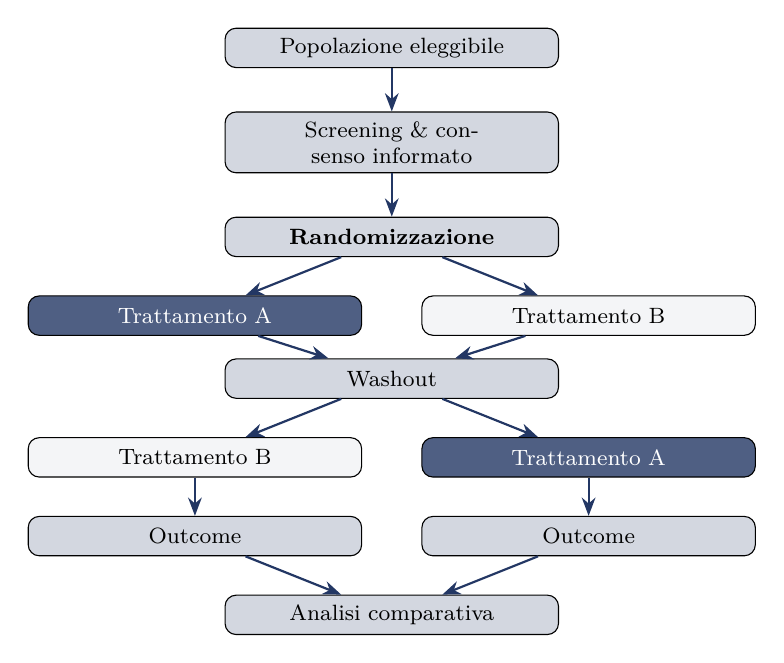
\begin{tikzpicture}[
  box/.style={draw, rounded corners, fill=mblue!20, text width=4cm,
  align=center, font=\footnotesize, minimum height=0.5cm},
  arr/.style={-{Stealth}, thick, mblue}
]
\node[box] (pop)  at (0, 4.2) {Popolazione eleggibile};
\node[box] (elig) at (0, 3.0) {Screening \& consenso informato};
\node[box] (rand) at (0, 1.8) {\textbf{Randomizzazione}};
\node[box, fill=mblue!80, text=white] (trt1A)  at (-2.5, 0.8) {Trattamento A};
\node[box, fill=mblue!05] (trt2B) at ( 2.5, 0.8) {Trattamento B};
\node[box] (wash)  at (0, 0) {Washout};
\node[box, fill=mblue!05] (trt1B)  at (-2.5, -1) {Trattamento B};
\node[box, fill=mblue!80, text=white] (trt2A) at ( 2.5, -1) {Trattamento A};
\node[box] (o1)   at (-2.5,-2) {Outcome};
\node[box] (o2)   at ( 2.5,-2) {Outcome};
\node[box] (anal) at (0,  -3) {Analisi comparativa};
\draw[arr] (pop)  -- (elig);
\draw[arr] (elig) -- (rand);
\draw[arr] (rand) -- (trt1A);
\draw[arr] (rand) -- (trt2B);
\draw[arr] (trt1A) -- (wash);
\draw[arr] (trt2B) -- (wash);
\draw[arr] (wash) -- (trt1B);
\draw[arr] (wash) -- (trt2A);
\draw[arr] (trt1B) -- (o1);
\draw[arr] (trt2A) -- (o2);
\draw[arr] (o1)   -- (anal);
\draw[arr] (o2)   -- (anal);
\end{tikzpicture}
\end{center}
\end{frame}

\begin{frame}{Disegno crossover: Note}
\phantomsection\label{disegno-crossover-note}
\small

\textbf{Vantaggi} - Ogni soggetto è controllo di sé stesso - Etico: ogni
soggetto sarà sottoposto a miglior trattamento

Importante tenere conto di:

\begin{itemize}
\tightlist
\item
  \textbf{Effetto periodo}: verificare se il tempo influenza i risultati
\item
  \textbf{Effetto sequenza}: considerare l'ordine dei trattamenti
  (A\(\to\)B vs B\(\to\)A)
\item
  \textbf{Effetto carryover}: controllare che il primo trattamento non
  influenzi il secondo
\item
  \textbf{Washout}: inserire periodo di ``washout'' tra trattamenti (può
  non essere possibile)
\end{itemize}
\end{frame}

\begin{frame}{RCT Non-inferiority design}
\phantomsection\label{rct-non-inferiority-design}
è un RCT in cui il controllo è il \emph{miglior trattamento disponibile}

\begin{center}
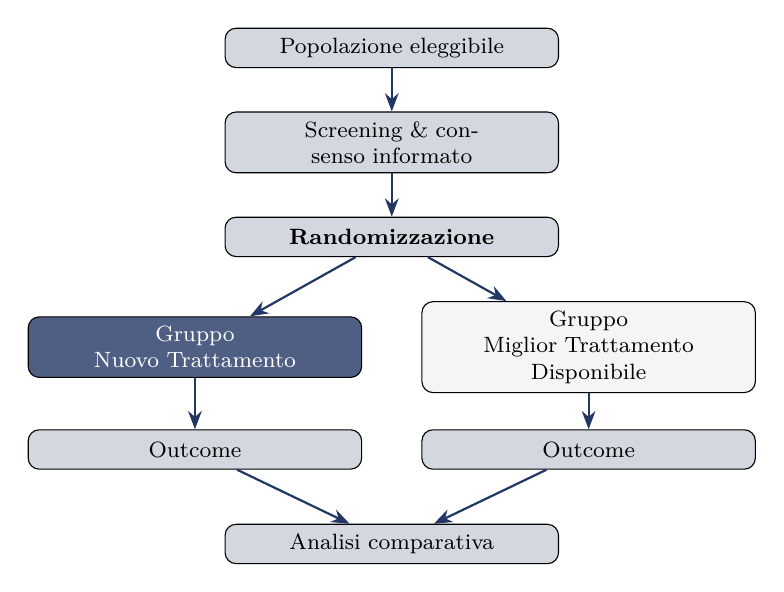
\begin{tikzpicture}[
  box/.style={draw, rounded corners, fill=mblue!20, text width=4cm,
  align=center, font=\footnotesize, minimum height=0.5cm},
  arr/.style={-{Stealth}, thick, mblue}
]
\node[box] (pop)  at (0, 4.2) {Popolazione eleggibile};
\node[box] (elig) at (0, 3.0) {Screening \& consenso informato};
\node[box] (rand) at (0, 1.8) {\textbf{Randomizzazione}};
\node[box, fill=mblue!80, text=white] (trt)  at (-2.5, 0.4) {Gruppo\\ Nuovo Trattamento};
\node[box, fill=mblue!05] (ctrl) at ( 2.5, 0.4) {Gruppo\\Miglior Trattamento\\ Disponibile};
\node[box] (o1)   at (-2.5,-0.9) {Outcome};
\node[box] (o2)   at ( 2.5,-0.9) {Outcome};
\node[box] (anal) at (0,  -2.1) {Analisi comparativa};
\draw[arr] (pop)  -- (elig);
\draw[arr] (elig) -- (rand);
\draw[arr] (rand) -- (trt);
\draw[arr] (rand) -- (ctrl);
\draw[arr] (trt)  -- (o1);
\draw[arr] (ctrl) -- (o2);
\draw[arr] (o1)   -- (anal);
\draw[arr] (o2)   -- (anal);
\end{tikzpicture}
\end{center}
\end{frame}

\begin{frame}{Disegno non-inferiority design: note}
\phantomsection\label{disegno-non-inferiority-design-note}
spesso è usato per proporre trattamenti più brevi/economici/meno
invasivi. è associato ad una tolleranza per considerare il trattamento
non inferiore.

\textbf{Vantaggi}:

\begin{itemize}
\tightlist
\item
  Etico: nessun gruppo non partecipa a nessun trattamento
\end{itemize}

Importante tenere conto di:

\begin{itemize}
\tightlist
\item
  Più difficile interpretare
\item
  Con una certa tolleranza, questi disegni potrebbero spingere verso
  trattamenti progressivamente peggiori.
\end{itemize}
\end{frame}

\begin{frame}{Tipologie di randomizzazione}
\phantomsection\label{tipologie-di-randomizzazione}
Esistono diversi tipi di modi di rifinire la randomizzazione

\begin{itemize}
\item
  \textbf{Stratified Randomization} alcune variabili rilevanti sono
  prese in considerazione, per evitare che i gruppi (tratt vs controllo)
  siano troppo sbilanciati.
\item
  \textbf{Cluster Randomization} ad essere randomizzati non sono i
  singoli individui, ma i cluster (es. tutti i pazienti di un ospedale
  fanno trattamento A, tutti i pazienti di un altro fanno trattamento
  B).
\item
  \ldots{} \vfill
\end{itemize}

vedi
\href{https://nata.kglmeridian.com/view/journals/attr/43/2/article-p215.xml}{\underline{\textbf{approfondimenti}}}
\end{frame}

\section{Disegni Quasi-Sperimentali}\label{disegni-quasi-sperimentali}

\begin{frame}{Disegni Quasi-Sperimentali: Interrupted Time Series}
\phantomsection\label{disegni-quasi-sperimentali-interrupted-time-series}
\begin{center}
\includegraphics[width=0.8\linewidth,height=\textheight,keepaspectratio]{Figures/Interrupted.png}
\end{center}
\end{frame}

\begin{frame}{Interrupted time series: note}
\phantomsection\label{interrupted-time-series-note}
\small Serie temporale di misure \textbf{prima e dopo} un intervento non
randomizzato. Si valutano cambiamenti di \textbf{livello} e/o
\textbf{pendenza}. Esempio: si monitora ripetutamente nel tempo un
paziente e poi si monitora dopo l'inizio del trattamento..
\end{frame}

\begin{frame}{Altri Disegni Quasi-Sperimentali}
\phantomsection\label{altri-disegni-quasi-sperimentali}
Esistono numerosi altri disegni quasi sperimentali.

\href{https://www.betterevaluation.org/sites/default/files/Quasi-Experimental_Design_and_Methods_ENG.pdf}{\underline{\textbf{Overview di disegni quasi sperimentali (Unicef)}}}

\href{https://pmc.ncbi.nlm.nih.gov/articles/PMC11741180/}{\underline{\textbf{Articolo su disegni quasi sperimentali}}}

\small
\end{frame}

\begin{frame}{Parentesi: Psicometria e sperimentazione clinica}
\phantomsection\label{parentesi-psicometria-e-sperimentazione-clinica}
Quale è il ruolo della psicometria (test e misure) nella sperimentazione
clinica? \pause

\textbf{Le inferenze cliniche in psicologia e neuropsicologia dipendono
enormemente dai test che utilizziamo}

Esempi:

\begin{itemize}
\tightlist
\item
  Potremmo non trovare effetti perchè i test hanno bassa affidabilità
\item
  Potremmo interpretare su base di \emph{face validity} ma non di reale
  \emph{validità di costrutto}
\end{itemize}
\end{frame}

\section{1.4 Selezione del Campione e Power
Statistico}\label{selezione-del-campione-e-power-statistico}

\begin{frame}{Selezione del Campione}
\phantomsection\label{selezione-del-campione}
\small

La \textbf{rappresentatività del campione} determina la
generalizzabilità dei risultati.

\vspace{0.4em}

\textbf{Criteri di inclusione/esclusione}: devono essere esplicitati e
giustificati teoricamente.

\begin{itemize}\footnotesize
\item Es.\ studio su MCI: età 60--85, scolarità $\geq$ 5 anni, assenza di depressione maggiore in atto, assenza di deficit sensoriali non corretti
\item Trade-off: campione omogeneo (validità interna) vs.\ eterogeneo (validità esterna)
\end{itemize}

\vspace{0.4em}
\end{frame}

\begin{frame}{Bias di selezione comuni in neuropsicologia/psicologia}
\phantomsection\label{bias-di-selezione-comuni-in-neuropsicologiapsicologia}
\begin{itemize}
\item \emph{Referral bias}: chi arriva in clinica non rappresenta la popolazione generale
\item \emph{Healthy volunteer bias}: chi si offre volontario è sistematicamente più sano
\item \emph{Survivorship bias}: nei longitudinali, chi abbandona non è un dropout casuale
\item \emph{WEIRD samples}: studi su popolazioni Western, Educated, Industrialized, Rich, Democratic
\end{itemize}
\end{frame}

\begin{frame}{Trade-off generalizzabile?}
\phantomsection\label{trade-off-generalizzabile}
In studi neuropsicologici spesso validità interna e validità esterna
sono in conflitto. All'aumentare della validità interna (campione
omogeneo per stabilire causa-effetto tra patologia e fenomeni di
interesse) diminuisce validità esterna (generalizzabilità dei
risultati).
\end{frame}

\begin{frame}{Convenience Sampling}
\phantomsection\label{convenience-sampling}
Spesso nei casi di studi psicologici il campione non è realmente un
\textbf{campione di convenienza} (campione a cui vi è facile accesso,
es. amici, colleghi, persone che si presentano al servizio).

Questa tipologia di campionamento pone limiti a generalizzabilità,
perché può introdurre \emph{bias}.
\end{frame}

\begin{frame}{Power (Potere Statistico)}
\phantomsection\label{power-potere-statistico}
\begin{center}
\includegraphics[width=0.7\linewidth,height=\textheight,keepaspectratio]{11-Disegni-di-Ricerca-Clinica_files/figure-beamer/unnamed-chunk-1-1.pdf}
\end{center}

\small Per \(\alpha = 0.05\), potere \(= 80\%\), effetto medio
(\(d = 0.5\)): circa 64 soggetti per gruppo. Gli studi neuropsicologici
sono spesso \textbf{underpowered} per effetti piccoli.
\end{frame}

\begin{frame}{Replication Crisis e Open Science}
\phantomsection\label{replication-crisis-e-open-science}
\small

\textbf{Il problema}: studi con N piccolo producono stime di effect size
instabili e sovrastimate (quando significative).

\vspace{0.3em}

\textbf{Open Science Collaboration (2015)}: 100 studi di psicologia
replicati --- solo \(\sim 36 \%\) ha ottenuto risultati significativi.

\vspace{0.4em}

\textbf{Soluzioni pratiche}:

\begin{itemize}\footnotesize
\item \textbf{Pre-registrazione}: ipotesi e analisi dichiarate prima di raccogliere i dati (ClinicalTrials.gov, OSF.io)
\item \textbf{Registered Reports}: la rivista accetta il paper \emph{prima} di vedere i risultati
\item \textbf{Open data e open materials}: riproducibilità delle analisi
\item \textbf{Multi-site studies}: aumentano la potenza e la generalizzabilità
\item Riportare sempre \textbf{effect size} e \textbf{intervalli di confidenza}, non solo il $p$-value
\end{itemize}

\vspace{0.2em}

\tiny Open Science Collaboration (2015). \emph{Science} 349(6251). Open
Access: \url{https://doi.org/10.1126/science.aac4716}
\end{frame}

\section{1.5 Machine Learning e Studi Predittivi
(Cenni)}\label{machine-learning-e-studi-predittivi-cenni}

\begin{frame}{ML in Ricerca Clinica}
\phantomsection\label{ml-in-ricerca-clinica}
\begin{center}
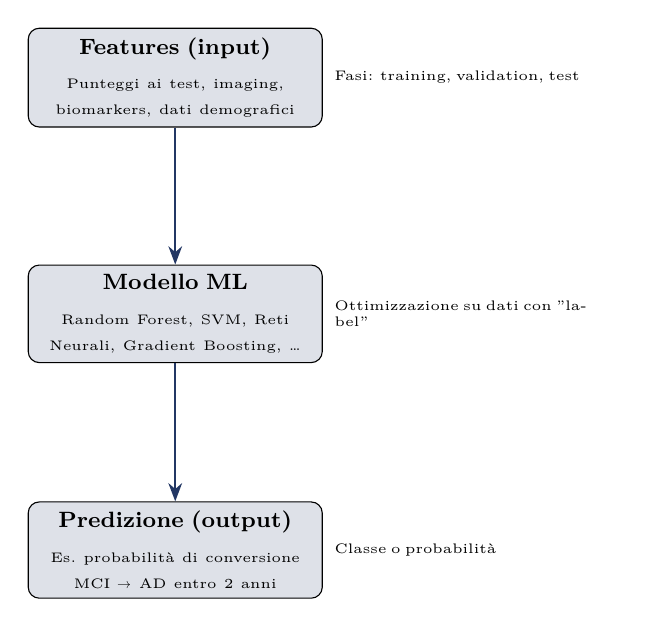
\begin{tikzpicture}[
  box/.style={draw, rounded corners, fill=mblue!15, text width=3.5cm,
  align=center, font=\footnotesize, minimum height=1.0cm},
  arr/.style={-{Stealth}, thick, mblue}
]
\node[box] (feat) at (0,3) {\textbf{Features (input)}\\[3pt]\tiny Punteggi ai test, imaging, biomarkers, dati demografici};
\node[box] (mod)  at (0,0) {\textbf{Modello ML}\\[3pt]\tiny Random Forest, SVM, Reti Neurali, Gradient Boosting, \ldots};
\node[box] (pred) at (0,-3) {\textbf{Predizione (output)}\\[3pt]\tiny Es.\ probabilità di conversione MCI $\to$ AD entro 2 anni};
\draw[arr] (feat) -- (mod);
\draw[arr] (mod)  -- (pred);
\node[right,font=\tiny,text width=3.5cm] at (1.9,3) {Fasi: training, validation, test};
\node[right,font=\tiny,text width=3.5cm] at (1.9,0) {Ottimizzazione su dati con "label"};
\node[right,font=\tiny,text width=3.5cm] at (1.9,-3) {Classe o probabilità};
\end{tikzpicture}
\end{center}
\end{frame}

\begin{frame}{ML vs Inferenza Classica}
\phantomsection\label{ml-vs-inferenza-classica}
\small

\begin{longtable}[]{@{}
  >{\raggedright\arraybackslash}p{(\linewidth - 4\tabcolsep) * \real{0.3333}}
  >{\raggedright\arraybackslash}p{(\linewidth - 4\tabcolsep) * \real{0.3333}}
  >{\raggedright\arraybackslash}p{(\linewidth - 4\tabcolsep) * \real{0.3333}}@{}}
\toprule\noalign{}
\begin{minipage}[b]{\linewidth}\raggedright
\end{minipage} & \begin{minipage}[b]{\linewidth}\raggedright
\textbf{Inferenza classica}
\end{minipage} & \begin{minipage}[b]{\linewidth}\raggedright
\textbf{Machine Learning}
\end{minipage} \\
\midrule\noalign{}
\endhead
\footnotesize Obiettivo & \footnotesize Testare ipotesi, spiegare &
\footnotesize Predire outcome \\
\footnotesize Focus & \footnotesize Parametri, \(p\)-value &
\footnotesize Accuratezza, AUC-ROC \\
\footnotesize Rischio principale & \footnotesize Falsi positivi (Type I)
& \footnotesize Overfitting \\
\footnotesize Validazione & \footnotesize Test statistici &
\footnotesize Cross-validation, hold-out \\
\footnotesize Interpretabilità & \footnotesize Alta &
\footnotesize Variabile (black box) \\
\bottomrule\noalign{}
\end{longtable}

\vspace{0.4em} \small \textbf{Attenzione}: un modello ML predice ma non
spiega meccanismi causali. Per interventi clinici serve anche una
comprensione causale (vedi prossime lezioni).

\vspace{0.2em}
\tiny Scandola et al. (2022). ML for brain disorders. \emph{NeuroImage}. \href{https://bpspsychub.onlinelibrary.wiley.com/doi/full/10.1111/jnp.70009}{\underline{\textbf{Download Article}}}
\end{frame}

\begin{frame}{ML: Principali problemi}
\phantomsection\label{ml-principali-problemi}
\small

\textbf{Overfitting}: il modello impara a memoria i dati di training, ma
non generalizza a nuovi dati.

\vspace{0.25em}

\textbf{Data leakage}: Alcuni dati esterni al ``training set'' filtrano
all'interno (in genere usando variabili sbagliate nella predizione)

\vspace{0.25em}

\textbf{Bias dei dati di training}: modello addestrato su popolazioni
non rappresentative (es.~solo caucasici anziani) non funziona su altri
gruppi.

\vspace{0.25em}

\textbf{Piccoli campioni in neuropsicologia}: molti studi ML pubblicati
hanno N troppo piccolo per una validazione robusta. Il numero di
features supera spesso il numero di soggetti (\(p \gg n\)).

\vspace{0.25em}

\textbf{Explainability}: molti modelli di ML sono di difficile
interpretabilità (es. \emph{``Importance''} non dice la direzione
dell'effetto di una variable, che può cambiare a seconda dei valori di
altri variabili).
\end{frame}

\section{Riepilogo}\label{riepilogo}

\begin{frame}{Riepilogo: Mappa dei Disegni}
\phantomsection\label{riepilogo-mappa-dei-disegni}
\begin{center}
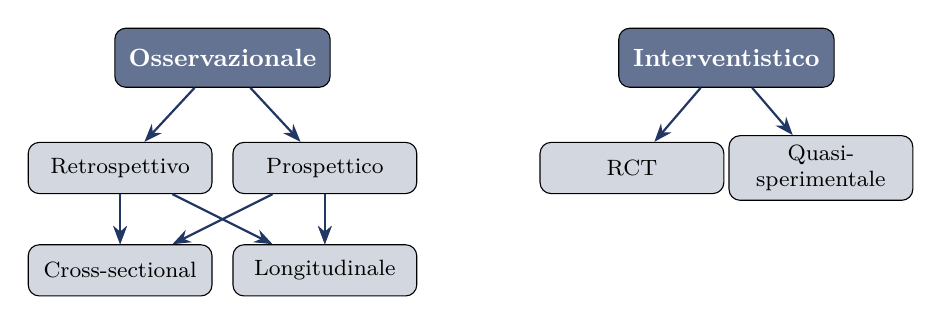
\begin{tikzpicture}[
  main/.style={draw, rounded corners, fill=mblue!70, text=white,
               font=\small\bfseries, text width=2.5cm, align=center, minimum height=0.75cm},
  sub/.style={draw, rounded corners, fill=mblue!20,
              font=\footnotesize, text width=2.1cm, align=center, minimum height=0.65cm},
  arr/.style={-{Stealth}, mblue, thick}
]
\node[main] (obs) at (-3.2, 3.0) {Osservazionale};
\node[main] (int) at ( 3.2, 3.0) {Interventistico};
\node[sub]  (ret) at (-4.5, 1.6) {Retrospettivo};
\node[sub]  (pro) at (-1.9, 1.6) {Prospettico};
\node[sub]  (cs)  at (-4.5, 0.3) {Cross-sectional};
\node[sub]  (lo)  at (-1.9, 0.3) {Longitudinale};
\node[sub]  (rct) at ( 2.0, 1.6) {RCT};
\node[sub]  (qe)  at ( 4.4, 1.6) {Quasi-sperimentale};
\draw[arr] (obs)--(ret); \draw[arr] (obs)--(pro);
\draw[arr] (ret)--(cs);  \draw[arr] (pro)--(lo);
\draw[arr] (ret)--(cs);  \draw[arr] (pro)--(lo);
\draw[arr] (ret)--(lo);  \draw[arr] (pro)--(cs);
\draw[arr] (int)--(rct); \draw[arr] (int)--(qe);
\end{tikzpicture}
\end{center}
\end{frame}




\end{document}
